% !TEX TS-program = lualatex
% !BIB TS-program = biber
%\documentclass[handout]{beamer}
\documentclass{beamer}
\input{../common/misomva}
%\newcommand{\misoclasstinytitleslide}{Partially based on material by:  Ulrike von Luxburg, \\[-1em] Gary Miller, Doyle \& Schnell, Daniel Spielman}
\newcommand{\misoclasstinytitleslide}{Partially based on material by:   Gary Miller, \\ Mikhail Belkin, Branislav Kveton, \\[-1em] Doyle \& Schnell, Daniel Spielman}
\newcommand{\misoclassdate}{}
\begin{document}
% Topic-specific title slide
\newcommand{\topictitle}{Semi-Supervised Learning Introduction}
\newcommand{\topicsubtitle}{Why and When SSL Helps}
\renewcommand{\misoclasstinytitleslide}{Partially based on material by:  Mikhail Belkin, Partha Niyogi, \\[-1em] Olivier Chapelle, Bernhard Sch\"olkopf}

\MakeTopicSlide

\begin{frame}
\frametitle{Semi-supervised learning: How is it possible?}
\begin{center}
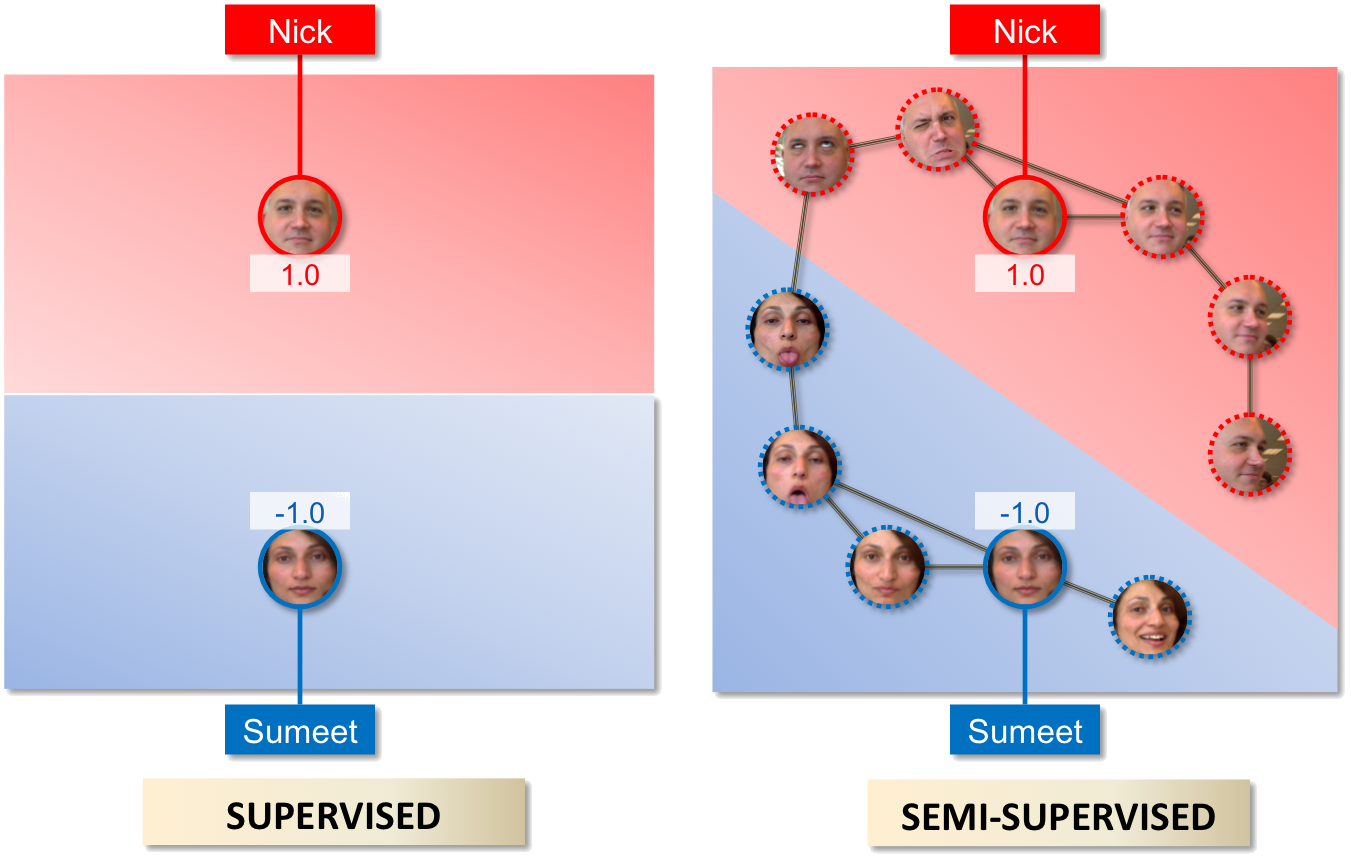
\includegraphics[width=0.9\columnwidth]{../img/ssl}
\end{center}
\pause
\rightyellbox{This is how children learn! \grcol{hypothesis}}

\end{frame}
%%%%%%%%%%%%%%%%%%%%%%%%%%%%%%%%%%%%%%%%%%%%%%%%%%%%%%%%%%%%
\begin{frame}
\frametitle{Semi-supervised learning (SSL)}

\begin{block}{SSL problem: definition}
\pause
Given $\{\bx_i\}_{i=1}^\nodes$ from $\R^d$ and 
$\{y_i\}_{i=1}^{n_l}$, with $n_l\ll \nodes$, find 
$\{y_i\}_{i=n_l+1}^\nodes$ (\textbf{transductive}) or find $f$ predicting 
$y$ well beyond that (\textbf{inductive}).
\end{block} 
\pause
\questionbox{Some facts about \gcol{SSL}}
\begin{itemize}%\addtolength{\itemsep}{0.25\baselineskip}
\item<+-> assumes that the unlabeled data is useful
\item<+-> works with data geometry assumptions
  \begin{itemize}
    \item cluster assumption --- low-density separation
    \item smoothness assumptions, generative models, \dots 
    \item manifold assumption
   \end{itemize}
\item<+-> now it helps now, now it does not (sic)
  \begin{itemize}
    \item provable cases when it helps
  \end{itemize}
 \item<+-> inductive or transductive/out-of-sample extension 
{\tiny \url{http://olivier.chapelle.cc/ssl-book/discussion.pdf}}
\end{itemize}

\end{frame}
%%%%%%%%%%%%%%%%%%%%%%%%%%%%%%%%%%%%%%%%%%%%%%%%%%%%%%%%%%%%

\begin{frame}
\frametitle{SSL: Overview: Self-Training}
\begin{block}{SSL: \gcol{Self-Training}}
\pause
\textbf{Input:} $\cL = \{\bx_i, y_i\}_{i=1}^{n_l}$ and 
$\cU = \{\bx_i\}_{i=n_l+1}^\nodes$ \\
\textbf{Repeat:}
  \begin{itemize}
    \item train $f$ using $\cL$
    \item apply $f$ to (some) $\cU$ and add them to $\cL$
  \end{itemize}
\end{block} 
\bigskip
\pause
\questionbox{What are the properties of self-training?}
\begin{itemize}[<+->]%\addtolength{\itemsep}{0.25\baselineskip}
\item its a wrapper method
\item heavily depends on the the internal classifier
\item some theory exist for specific classifiers
\item nobody uses it anymore ($\neq$ self supervised)
\item errors propagate (unless the clusters are well separated)
\end{itemize} 
\end{frame}
 
\begin{frame}
\frametitle{SSL: Self-Training (Good Case)}

\begin{center}
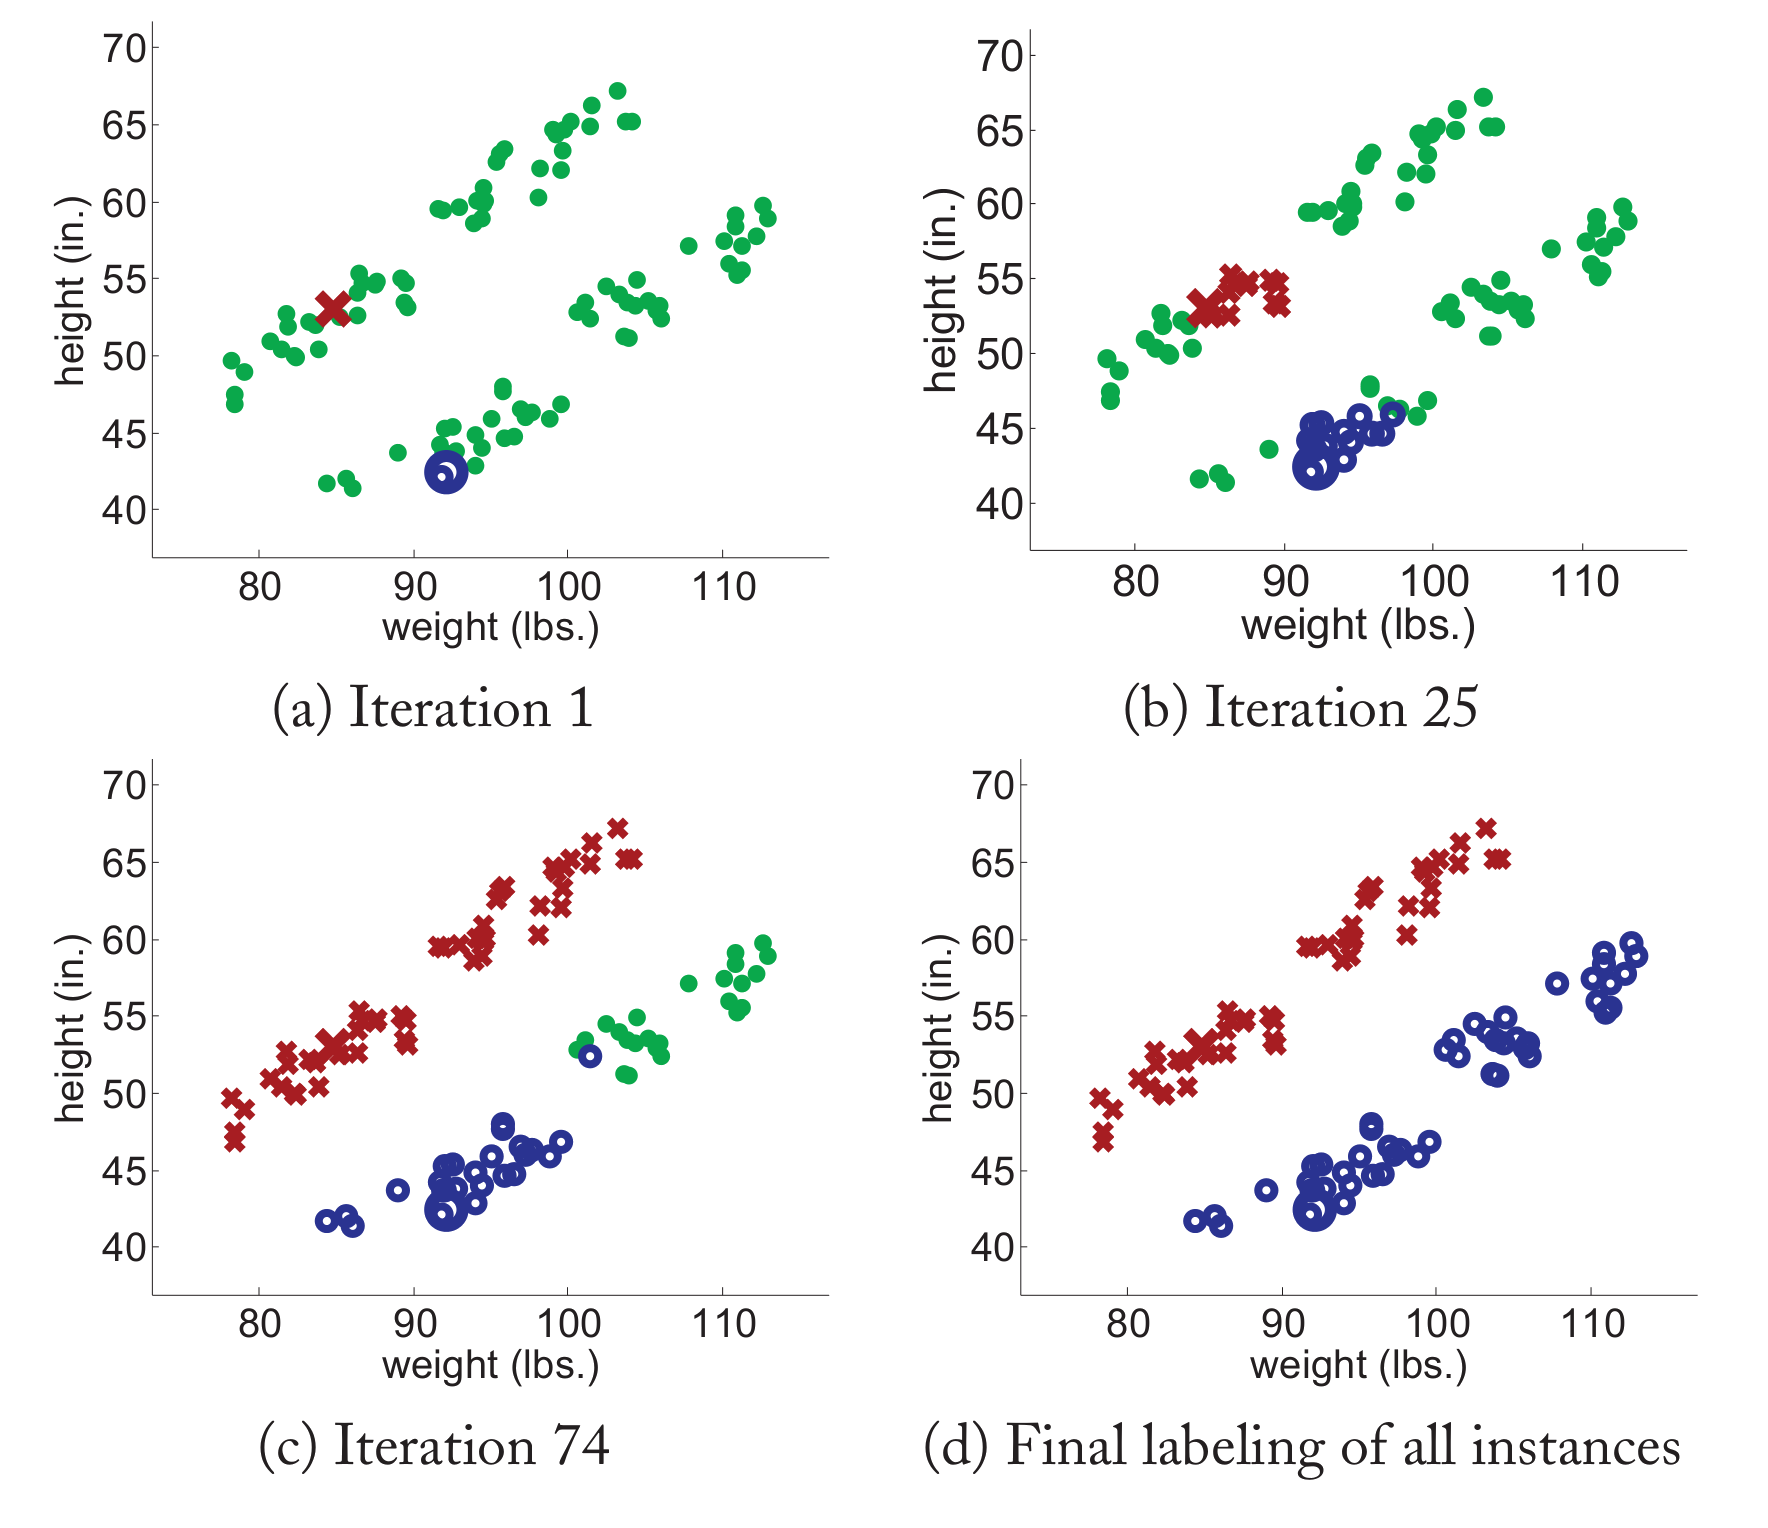
\includegraphics[width=0.8\columnwidth, height=0.65\textheight, keepaspectratio]{../img/self}
\\[0.5em] {\tiny Source: \citet{chapelle2006semi-supervised}}
\end{center}

\end{frame}
%%%%%%%%%%%%%%%%%%%%%%%%%%%%%%%%%%%%%%%%%%%%%%%%%%%%%%%%%%%%
\begin{frame}
\frametitle{SSL: Self-Training (Bad Case)}

\begin{center}
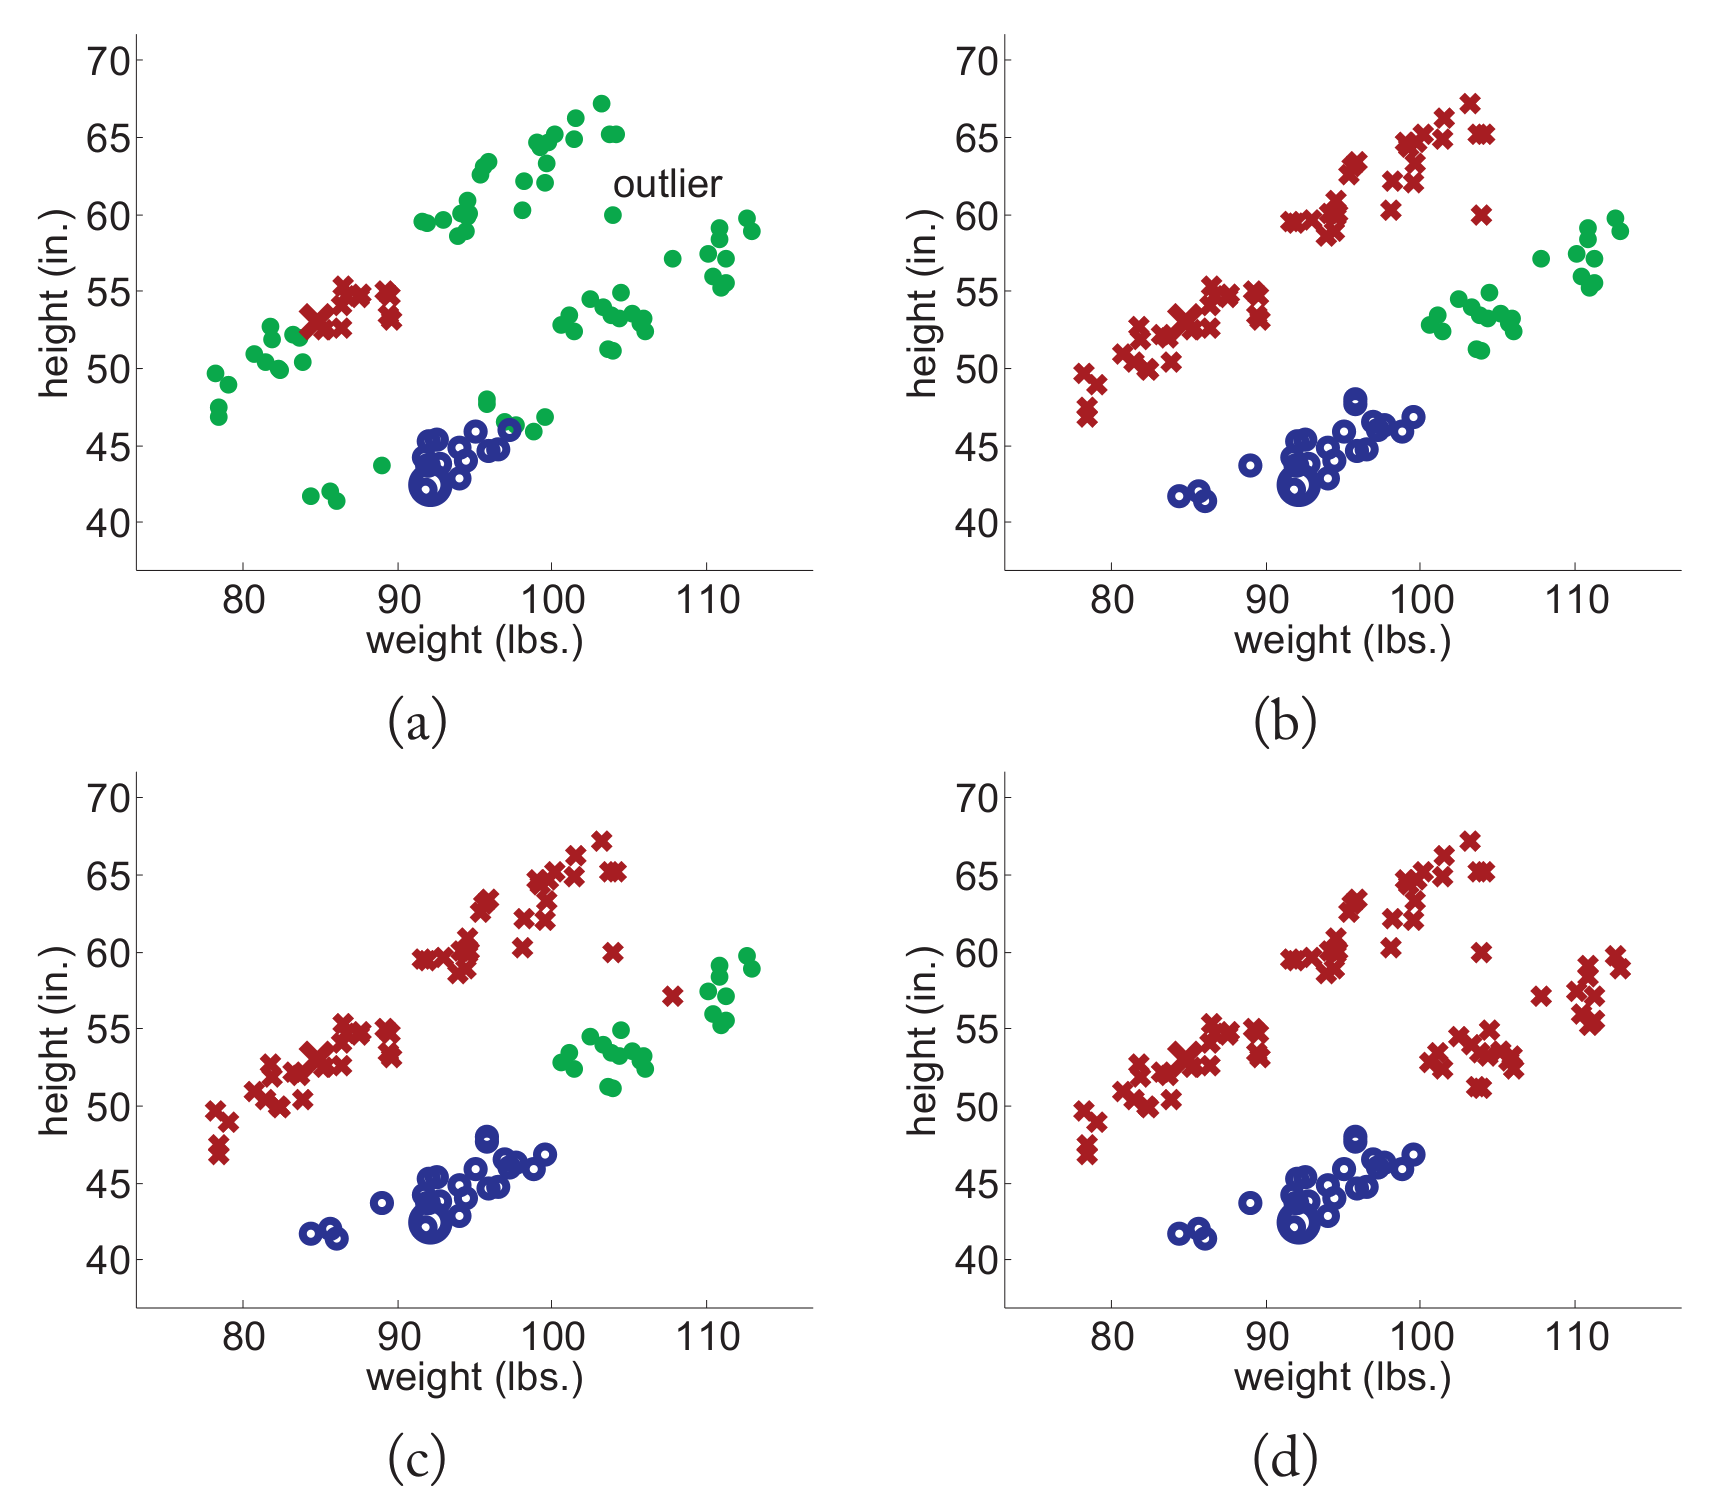
\includegraphics[width=0.8\columnwidth, height=0.65\textheight, keepaspectratio]{../img/self2}
\\[0.5em] {\tiny Source: \citet{chapelle2006semi-supervised}}
\end{center}
\end{frame}

%%%%%%%%%%%%%%%%%%%%%%%%%%%%%%%%%%%%%%%%%%%%%%%%%%%%%%%%%%%%

\setbeamercolor{background canvas}{bg=vert1}
\setbeamertemplate{background canvas}[default] 
\setbeamertemplate{footline}{
\hspace{2cm}  \raisebox{2.5ex}
 % {{EMETTEUR - NOM DE LA PRESENTATION}}\hfill 
    {{}}\hfill 
  \raisebox{2.5ex}
  %{{\today - \insertframenumber \hspace{5mm} \null }}}
  {{ \null }}}
\begin{frame}\begin{textblock*}{10cm}(13mm,40mm)
{\textcolor{white} {
{\monster {\bf SSL}$(\cG)$}\\[2mm]
   { \huge semi-supervised learning  with graphs and harmonic functions}\\[3mm]
   	%{\Large Sous-titre facultatif}}
	{\Large \dots our running example for learning with graphs}}}
	\end{textblock*}
\vspace*{-4pt}\end{frame}\MakeNormalSlide

%%%%%%%%%%%%%%%%%%%%%%%%%%%%%%%%%%%%%%%%%%%%%%%%%%%%%%%%%%%%
%%%%%%%%%%%%%%%%%%%%%%%%%%%%%%%%%%%%%%%%%%%%%%%%%%%%%%%%%%%%
\begin{frame}
\frametitle{SSL with Graphs: Prehistory}

{\footnotesize Blum/Chawla: Learning from Labeled and Unlabeled Data using Graph Mincuts}\\
{\scriptsize \url{http://www.aladdin.cs.cmu.edu/papers/pdfs/y2001/mincut.pdf} \\
\pause
\notecol{*following some insights from vision research in 1980s }
}

\pause

\begin{center}
\resizebox{0.7\columnwidth}{!}{%
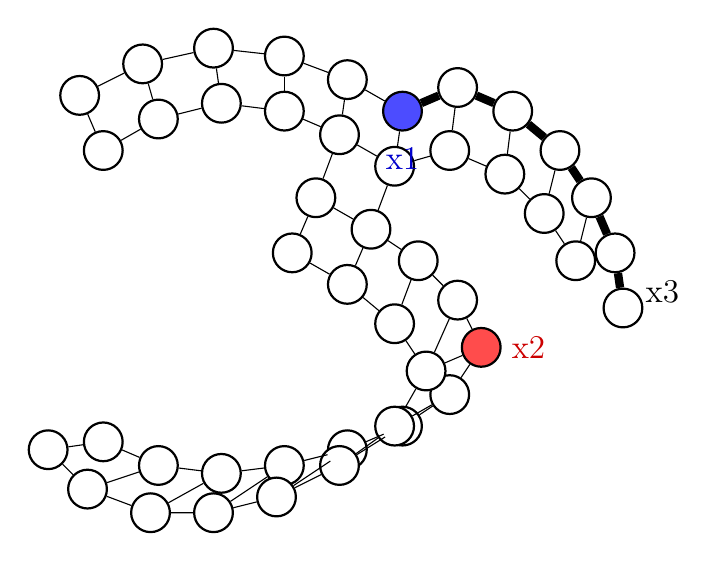
\begin{tikzpicture}[
    unlabeled/.style={circle, draw=black, thick, minimum size=14pt, fill=white},
    positive/.style={circle, draw=black, thick, minimum size=14pt, fill=blue!70},
    negative/.style={circle, draw=black, thick, minimum size=14pt, fill=red!70},
    edge/.style={draw=black, thin},
    cut/.style={draw=black, line width=3pt}
]

    % === Upper arc - outer row (top curve going left to right then down) ===
    \node[unlabeled] (a1) at (0.5, 4.5) {};
    \node[unlabeled] (a2) at (1.3, 4.9) {};
    \node[unlabeled] (a3) at (2.2, 5.1) {};
    \node[unlabeled] (a4) at (3.1, 5.0) {};
    \node[unlabeled] (a5) at (3.9, 4.7) {};
    \node[positive] (x1) at (4.6, 4.3) {};  % Blue node x1
    \node[unlabeled] (a6) at (5.3, 4.6) {};
    \node[unlabeled] (a7) at (6.0, 4.3) {};
    \node[unlabeled] (a8) at (6.6, 3.8) {};
    \node[unlabeled] (a9) at (7.0, 3.2) {};
    \node[unlabeled] (a10) at (7.3, 2.5) {};
    \node[unlabeled] (a11) at (7.4, 1.8) {};
    
    % Upper arc - inner row
    \node[unlabeled] (b1) at (0.8, 3.8) {};
    \node[unlabeled] (b2) at (1.5, 4.2) {};
    \node[unlabeled] (b3) at (2.3, 4.4) {};
    \node[unlabeled] (b4) at (3.1, 4.3) {};
    \node[unlabeled] (b5) at (3.8, 4.0) {};
    \node[unlabeled] (b6) at (4.5, 3.6) {};
    \node[unlabeled] (b7) at (5.2, 3.8) {};
    \node[unlabeled] (b8) at (5.9, 3.5) {};
    \node[unlabeled] (b9) at (6.4, 3.0) {};
    \node[unlabeled] (b10) at (6.8, 2.4) {};
    
    % Edges - upper arc outer
    \draw[edge] (a1) -- (a2) -- (a3) -- (a4) -- (a5) -- (x1);
    \draw[cut] (x1) -- (a6);  % Bold edge from x1
    \draw[cut] (a6) -- (a7);  % Bold edge (continuous path)
    \draw[cut] (a7) -- (a8);  % Bold edge (cut)
    \draw[cut] (a8) -- (a9);  % Bold edge (cut)
    \draw[cut] (a9) -- (a10);  % Bold edge to x3
    \draw[cut] (a10) -- (a11);  % Bold edge to x3
    
    % Edges - upper arc inner
    \draw[edge] (b1) -- (b2) -- (b3) -- (b4) -- (b5) -- (b6) -- (b7) -- (b8);
    \draw[edge] (b8) -- (b9);
    \draw[edge] (b9) -- (b10);
    
    % Cross edges upper arc
    \draw[edge] (a1) -- (b1);
    \draw[edge] (a2) -- (b2);
    \draw[edge] (a3) -- (b3);
    \draw[edge] (a4) -- (b4);
    \draw[edge] (a5) -- (b5);
    \draw[edge] (x1) -- (b6);
    \draw[edge] (a6) -- (b7);
    \draw[edge] (a7) -- (b8);
    \draw[edge] (a8) -- (b9);
    \draw[edge] (a9) -- (b10);
    \draw[edge] (a10) -- (b10);
    
    % === Lower arc - inner row (from middle going down-left) ===
    \node[unlabeled] (c1) at (3.5, 3.2) {};
    \node[unlabeled] (c2) at (4.2, 2.8) {};
    \node[unlabeled] (c3) at (4.8, 2.4) {};
    \node[unlabeled] (c4) at (5.3, 1.9) {};
    \node[negative] (x2) at (5.6, 1.3) {};  % Red node x2
    \node[unlabeled] (c5) at (5.2, 0.7) {};
    \node[unlabeled] (c6) at (4.6, 0.3) {};
    \node[unlabeled] (c7) at (3.9, 0.0) {};
    \node[unlabeled] (c8) at (3.1, -0.2) {};
    \node[unlabeled] (c9) at (2.3, -0.3) {};
    \node[unlabeled] (c10) at (1.5, -0.2) {};
    \node[unlabeled] (c11) at (0.8, 0.1) {};
    
    % Lower arc - outer row
    \node[unlabeled] (d1) at (3.2, 2.5) {};
    \node[unlabeled] (d2) at (3.9, 2.1) {};
    \node[unlabeled] (d3) at (4.5, 1.6) {};
    \node[unlabeled] (d4) at (4.9, 1.0) {};
    \node[unlabeled] (d5) at (4.5, 0.3) {};
    \node[unlabeled] (d6) at (3.8, -0.2) {};
    \node[unlabeled] (d7) at (3.0, -0.6) {};
    \node[unlabeled] (d8) at (2.2, -0.8) {};
    \node[unlabeled] (d9) at (1.4, -0.8) {};
    \node[unlabeled] (d10) at (0.6, -0.5) {};
    \node[unlabeled] (d11) at (0.1, 0.0) {};
    
    % Edges - lower arc inner
    \draw[edge] (c1) -- (c2) -- (c3) -- (c4) -- (x2) -- (c5) -- (c6) -- (c7) -- (c8) -- (c9) -- (c10) -- (c11);
    
    % Edges - lower arc outer
    \draw[edge] (d1) -- (d2) -- (d3) -- (d4) -- (d5) -- (d6) -- (d7) -- (d8) -- (d9) -- (d10) -- (d11);
    
    % Cross edges lower arc
    \draw[edge] (c1) -- (d1);
    \draw[edge] (c2) -- (d2);
    \draw[edge] (c3) -- (d3);
    \draw[edge] (c4) -- (d4);
    \draw[edge] (x2) -- (d4);
    \draw[edge] (c5) -- (d5);
    \draw[edge] (c6) -- (d6);
    \draw[edge] (c7) -- (d7);
    \draw[edge] (c8) -- (d8);
    \draw[edge] (c9) -- (d9);
    \draw[edge] (c10) -- (d10);
    \draw[edge] (c11) -- (d11);
    
    % Connection between upper and lower arcs
    \draw[edge] (c1) -- (b5);
    \draw[edge] (c2) -- (b6);
    
    % Labels
    \node[blue!80!black, font=\large] at (4.6, 3.7) {x1};
    \node[red!80!black, font=\large] at (6.2, 1.3) {x2};
    \node[font=\large] at (7.9, 2.0) {x3};
    
\end{tikzpicture}
}
\end{center}
\end{frame}
%%%%%%%%%%%%%%%%%%%%%%%%%%%%%%%%%%%%%%%%%%%%%%%%%%%%%%%%%%%%
\begin{frame}
\frametitle{SSL with Graphs: MinCut}
\begin{center}
\resizebox{0.3\columnwidth}{!}{%
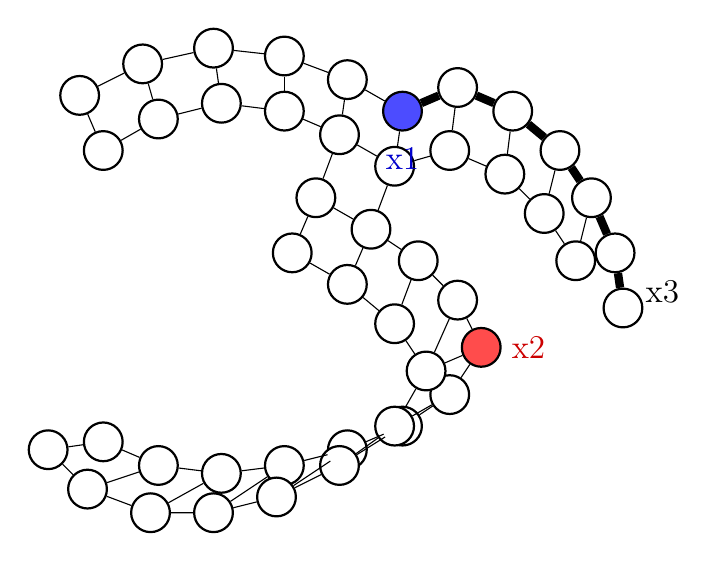
\begin{tikzpicture}[
    unlabeled/.style={circle, draw=black, thick, minimum size=14pt, fill=white},
    positive/.style={circle, draw=black, thick, minimum size=14pt, fill=blue!70},
    negative/.style={circle, draw=black, thick, minimum size=14pt, fill=red!70},
    edge/.style={draw=black, thin},
    cut/.style={draw=black, line width=3pt}
]

    % === Upper arc - outer row (top curve going left to right then down) ===
    \node[unlabeled] (a1) at (0.5, 4.5) {};
    \node[unlabeled] (a2) at (1.3, 4.9) {};
    \node[unlabeled] (a3) at (2.2, 5.1) {};
    \node[unlabeled] (a4) at (3.1, 5.0) {};
    \node[unlabeled] (a5) at (3.9, 4.7) {};
    \node[positive] (x1) at (4.6, 4.3) {};  % Blue node x1
    \node[unlabeled] (a6) at (5.3, 4.6) {};
    \node[unlabeled] (a7) at (6.0, 4.3) {};
    \node[unlabeled] (a8) at (6.6, 3.8) {};
    \node[unlabeled] (a9) at (7.0, 3.2) {};
    \node[unlabeled] (a10) at (7.3, 2.5) {};
    \node[unlabeled] (a11) at (7.4, 1.8) {};
    
    % Upper arc - inner row
    \node[unlabeled] (b1) at (0.8, 3.8) {};
    \node[unlabeled] (b2) at (1.5, 4.2) {};
    \node[unlabeled] (b3) at (2.3, 4.4) {};
    \node[unlabeled] (b4) at (3.1, 4.3) {};
    \node[unlabeled] (b5) at (3.8, 4.0) {};
    \node[unlabeled] (b6) at (4.5, 3.6) {};
    \node[unlabeled] (b7) at (5.2, 3.8) {};
    \node[unlabeled] (b8) at (5.9, 3.5) {};
    \node[unlabeled] (b9) at (6.4, 3.0) {};
    \node[unlabeled] (b10) at (6.8, 2.4) {};
    
    % Edges - upper arc outer
    \draw[edge] (a1) -- (a2) -- (a3) -- (a4) -- (a5) -- (x1);
    \draw[cut] (x1) -- (a6);  % Bold edge from x1
    \draw[cut] (a6) -- (a7);  % Bold edge (continuous path)
    \draw[cut] (a7) -- (a8);  % Bold edge (cut)
    \draw[cut] (a8) -- (a9);  % Bold edge (cut)
    \draw[cut] (a9) -- (a10);  % Bold edge to x3
    \draw[cut] (a10) -- (a11);  % Bold edge to x3
    
    % Edges - upper arc inner
    \draw[edge] (b1) -- (b2) -- (b3) -- (b4) -- (b5) -- (b6) -- (b7) -- (b8);
    \draw[edge] (b8) -- (b9);
    \draw[edge] (b9) -- (b10);
    
    % Cross edges upper arc
    \draw[edge] (a1) -- (b1);
    \draw[edge] (a2) -- (b2);
    \draw[edge] (a3) -- (b3);
    \draw[edge] (a4) -- (b4);
    \draw[edge] (a5) -- (b5);
    \draw[edge] (x1) -- (b6);
    \draw[edge] (a6) -- (b7);
    \draw[edge] (a7) -- (b8);
    \draw[edge] (a8) -- (b9);
    \draw[edge] (a9) -- (b10);
    \draw[edge] (a10) -- (b10);
    
    % === Lower arc - inner row (from middle going down-left) ===
    \node[unlabeled] (c1) at (3.5, 3.2) {};
    \node[unlabeled] (c2) at (4.2, 2.8) {};
    \node[unlabeled] (c3) at (4.8, 2.4) {};
    \node[unlabeled] (c4) at (5.3, 1.9) {};
    \node[negative] (x2) at (5.6, 1.3) {};  % Red node x2
    \node[unlabeled] (c5) at (5.2, 0.7) {};
    \node[unlabeled] (c6) at (4.6, 0.3) {};
    \node[unlabeled] (c7) at (3.9, 0.0) {};
    \node[unlabeled] (c8) at (3.1, -0.2) {};
    \node[unlabeled] (c9) at (2.3, -0.3) {};
    \node[unlabeled] (c10) at (1.5, -0.2) {};
    \node[unlabeled] (c11) at (0.8, 0.1) {};
    
    % Lower arc - outer row
    \node[unlabeled] (d1) at (3.2, 2.5) {};
    \node[unlabeled] (d2) at (3.9, 2.1) {};
    \node[unlabeled] (d3) at (4.5, 1.6) {};
    \node[unlabeled] (d4) at (4.9, 1.0) {};
    \node[unlabeled] (d5) at (4.5, 0.3) {};
    \node[unlabeled] (d6) at (3.8, -0.2) {};
    \node[unlabeled] (d7) at (3.0, -0.6) {};
    \node[unlabeled] (d8) at (2.2, -0.8) {};
    \node[unlabeled] (d9) at (1.4, -0.8) {};
    \node[unlabeled] (d10) at (0.6, -0.5) {};
    \node[unlabeled] (d11) at (0.1, 0.0) {};
    
    % Edges - lower arc inner
    \draw[edge] (c1) -- (c2) -- (c3) -- (c4) -- (x2) -- (c5) -- (c6) -- (c7) -- (c8) -- (c9) -- (c10) -- (c11);
    
    % Edges - lower arc outer
    \draw[edge] (d1) -- (d2) -- (d3) -- (d4) -- (d5) -- (d6) -- (d7) -- (d8) -- (d9) -- (d10) -- (d11);
    
    % Cross edges lower arc
    \draw[edge] (c1) -- (d1);
    \draw[edge] (c2) -- (d2);
    \draw[edge] (c3) -- (d3);
    \draw[edge] (c4) -- (d4);
    \draw[edge] (x2) -- (d4);
    \draw[edge] (c5) -- (d5);
    \draw[edge] (c6) -- (d6);
    \draw[edge] (c7) -- (d7);
    \draw[edge] (c8) -- (d8);
    \draw[edge] (c9) -- (d9);
    \draw[edge] (c10) -- (d10);
    \draw[edge] (c11) -- (d11);
    
    % Connection between upper and lower arcs
    \draw[edge] (c1) -- (b5);
    \draw[edge] (c2) -- (b6);
    
    % Labels
    \node[blue!80!black, font=\large] at (4.6, 3.7) {x1};
    \node[red!80!black, font=\large] at (6.2, 1.3) {x2};
    \node[font=\large] at (7.9, 2.0) {x3};
    
\end{tikzpicture}
}
\end{center}
\vskip -1em
\textbf{MinCut SSL}: an idea similar to MinCut clustering
\pause
\questionbox{Where is the link?} 
\pause 
\onslide<handout:0>{\notecol{%
connected classes, not necessarily compact}}
\pause 
\\ \smallskip
\questionbox{What is the formal statement?} 
\pause 
We look for $f(\bx) \in \{\pm 1\}$ 
\[
{\rm cut} = \pause\sum_{i,j=1}^{n_l+n_u}  w_{ij}  \left( f(\bx_i)  - f(\bx_j)  \right)^2
\pause = \Omega(f) 
\]
\vskip -1em
\pause
\questionbox{ Why $\left( f\left(\bx_i\right)  - f\left(\bx_j\right)  \right)^2$ and not 
$\left| f(\bx_i)  - f(\bx_j)  \right|$?} \pause 
\onslide<handout:0>{\notecol{%
{\tiny It does not matter.}}}

\end{frame}
%%%%%%%%%%%%%%%%%%%%%%%%%%%%%%%%%%%%%%%%%%%%%%%%%%%%%%%%%%%%
\begin{frame}
\frametitle{SSL with Graphs: MinCut}
We look for $f(\bx) \in \{\pm 1\}$  to minimize the cut $\Omega(\bff)$ 
\[
\Omega(\bff)  =  \sum_{i,j=1}^{n_l+n_u} w_{ij} \left( f(\bx_i)  - f(\bx_j)  \right)^2
\]
\pause
\rightyellbox{Clustering was unsupervised, here we have supervised data.}
\pause
Recall the general objective-function framework:
\[
 \min_{\bw, b}  \sum_i^{n_l} \mcolA{V(\bx_i, y_i, f\left( \bx_i \right))} + \lambda 
\mcolB{\Omega(\bff)}
\]
\pause
It would be nice if we match the prediction on labeled data:
\[
 \mcolA{V(\bx, y, f\left( \bx \right))} \pause = \only<6>{\alert{\infty}} \sum_{i=1}^{n_l} \left( f(\bx_i) - y_i \right)^2
\]

\end{frame}
%%%%%%%%%%%%%%%%%%%%%%%%%%%%%%%%%%%%%%%%%%%%%%%%%%%%%%%%%%%%
\begin{frame}
\frametitle{SSL with Graphs: MinCut}
\pause
Final objective function:
\[
 \min_{\bff  \in \{\pm 1\}^{n_l + n_u} }\mcolA{\infty \sum_{i=1}^{n_l} \left( f(\bx_i) - y_i \right)^2}
 + \lambda\mcolB{\sum_{i,j=1}^{n_l+n_u} w_{ij} \left( f(\bx_i)  - f(\bx_j)  \right)^2}
\]
\pause
\vskip -1em
\rightyellbox{This is an integer program :(}
\pause
\questionbox{Can we solve it?} 
\pause
\onslide<handout:0>{\notecol{%
It still just MinCut.}}
$\quad$
\pause
\questionbox{Are we happy?}
\pause
\begin{center}
% Min-cut bad example - TikZ replacement
\begin{tikzpicture}[
    vertex/.style={circle, draw=black, thick, minimum size=12pt, inner sep=0pt}
]
    \def\sp{1.0}
    \foreach \i in {0,\dots,6} {
        \node[vertex] (v\i) at (\i*\sp, 0) {};
    }
    \foreach \i in {0,\dots,5} {
        \pgfmathtruncatemacro{\j}{\i+1}
        \draw[thick] (v\i) -- (v\j);
    }
    \node[font=\Large\bfseries] at (-0.5, -0.6) {$+$};
    \node[font=\Large\bfseries] at (6.5, -0.6) {$-$};
\end{tikzpicture}
\end{center}
\vskip -1em
\pause 
\onslide<handout:0>{\notecol{%
There are six solutions.}}
\pause 
\onslide<handout:0>{\notecol{%
All equivalent.}}
\\
\pause 
\begin{flushright}
\emphcol{We need a better way to reflect the confidence.}
\end{flushright}
\end{frame}


\MakeLastSlide
\end{document}
